
In this chapter, we will outline the methodology used to train Bayesian neural networks. We will commence with a description of the dataset and the transformations employed on the datapoints. We will then briefly explain the training methodology employed with a discussion of the implementation and performance metrics to be used for testing of the trained models.

\section{The Dataset}\label{sec:dataset}
In this section, we will give a brief description of the dataset. Moreover, we will discuss the data transformations prior to training and its implications on the accuracy of the predictions.

For the predictions presented in this chapter, we have restricted our investigations to use the dataset for a single particle production process throughout. This will make it easier to compare the performance of BNNs across different configurations to better understand the strengths and weaknesses of the different choices made when training BNNs. 

\subsection{The Features and Targets}
We will focus on a particular neutralino-neutralino. Neuralinos are denoted by the symbol $\tilde{\chi}_i^0$ for $i = 1, 2, 3, 4$.
Each neutralino carries its own \textit{mass} $m_{\tilde{\chi}_i}$ and a set of \textit{mixing angles} $N_{ij}$ expressing the strength of its coupling to other particles. For each neutralino $i$, there are four mixing angles for $j = 1, 2, 3, 4$. The two possible cases of interest then would be a process with two identical neutralinos in the final state, in which case the input features are of the form
\begin{equation}\label{eq:neutralino_feat}
    x = (m_{\tilde{\chi}_i^0}, N_{i1}, N_{i2}, N_{i3}, N_{i4}),
\end{equation} 
or a process where there are two distinct neutralinos $i$ and $k$ in the final state, such that the input features would have the form
\begin{equation}
    x = (m_{\tilde{\chi}_i}^0, N_{i1}, N_{i2}, N_{i3}, N_{i4}, m_{\tilde{\chi}_k^0},  N_{k1}, N_{k2}, N_{k3}, N_{k4}).
\end{equation}
The targets of the dataset are NLO cross sections of the form
\begin{equation}
    \sigma_{\tilde{\chi}_i^0 \tilde{\chi}_k^0} = \text{LO} + \text{NLO}.
\end{equation}
In our case we will focus on processes that results in $\tilde{\chi}_1^0\tilde{\chi}_1^0$, meaning the input features have the form in eq.~\eqref{eq:neutralino_feat}. The masses $m_{\tilde{\chi}_i^0}$ can take on both postive and negative values in the dataset. 

In figure \ref{fig:dataset_masses}, we show the NLO cross sections $\sigma_{\tilde{\chi}_1^0 \tilde{\chi}_1^0}$ for points taken from the training set projected onto the axis of masses $m_{\tilde{\chi}_1^0}$ and in figure \ref{fig:dataset_mixing_angles} we show their values projected onto the axes of the mixing angles $N_{1j}$ for $j=1,2,3,4$. 
Note in particular that the cross sections span several orders of magnitude which necessitates a data transformation to reliably perform regression analysis with the dataset. We can also note a few outliers most of which yield neglible cross section values, but we should be aware of that adverse effect of these can affect the trained BNN models. There is a certain asymmetry in some of the features as well, where there are largely more cross sections on the right side of $m_{\tilde{\chi}_1^0}$ which may bias the weights of the BNN to perform better if the its input contain a positive mass. We can observe a similar asymmetry for $N_{11}$ and $N_{13}$ in figure \ref{fig:dataset_mixing_angles}. It is worth noting that cross sections with very low values come from a fine tuned region where $N_{11}$ and $N_{12}$ are approximately zero.


\begin{figure}[h!]
    \centering
    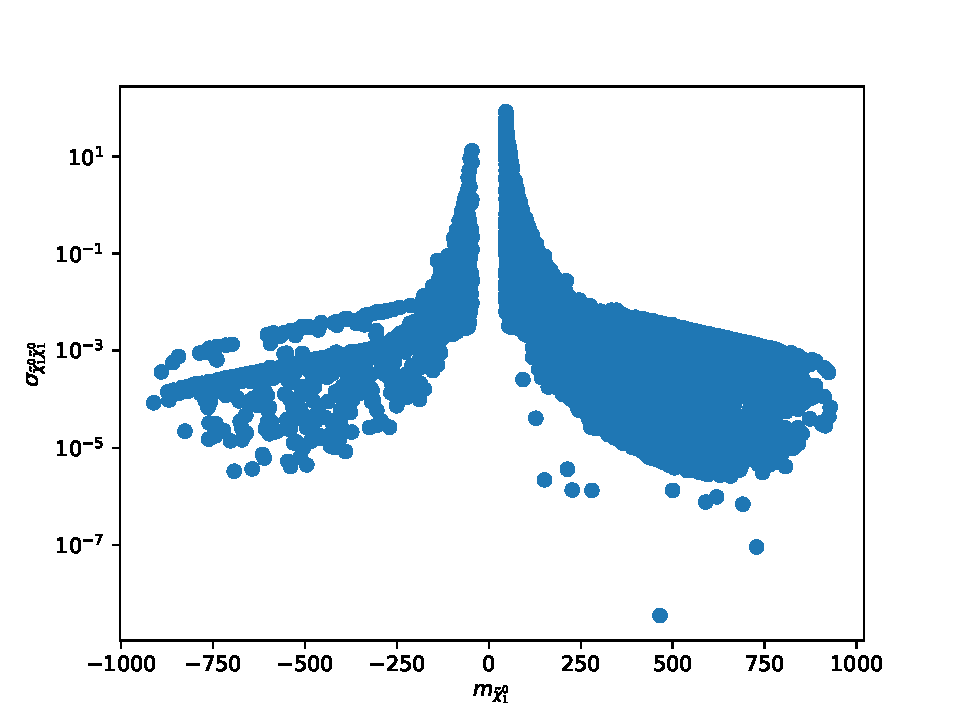
\includegraphics[scale=0.7]{figures/dataset/masses.pdf}
    \caption{The values of the cross sections $\sigma_{\tilde{\chi}_1^0 \tilde{\chi}_1^0}$ are shown projected onto the axis of masses $m_{\tilde{\chi}_1^0}$. The data is taken from the training data.
    }\label{fig:dataset_masses}
\end{figure}


\begin{figure}[h!]
    \centering
    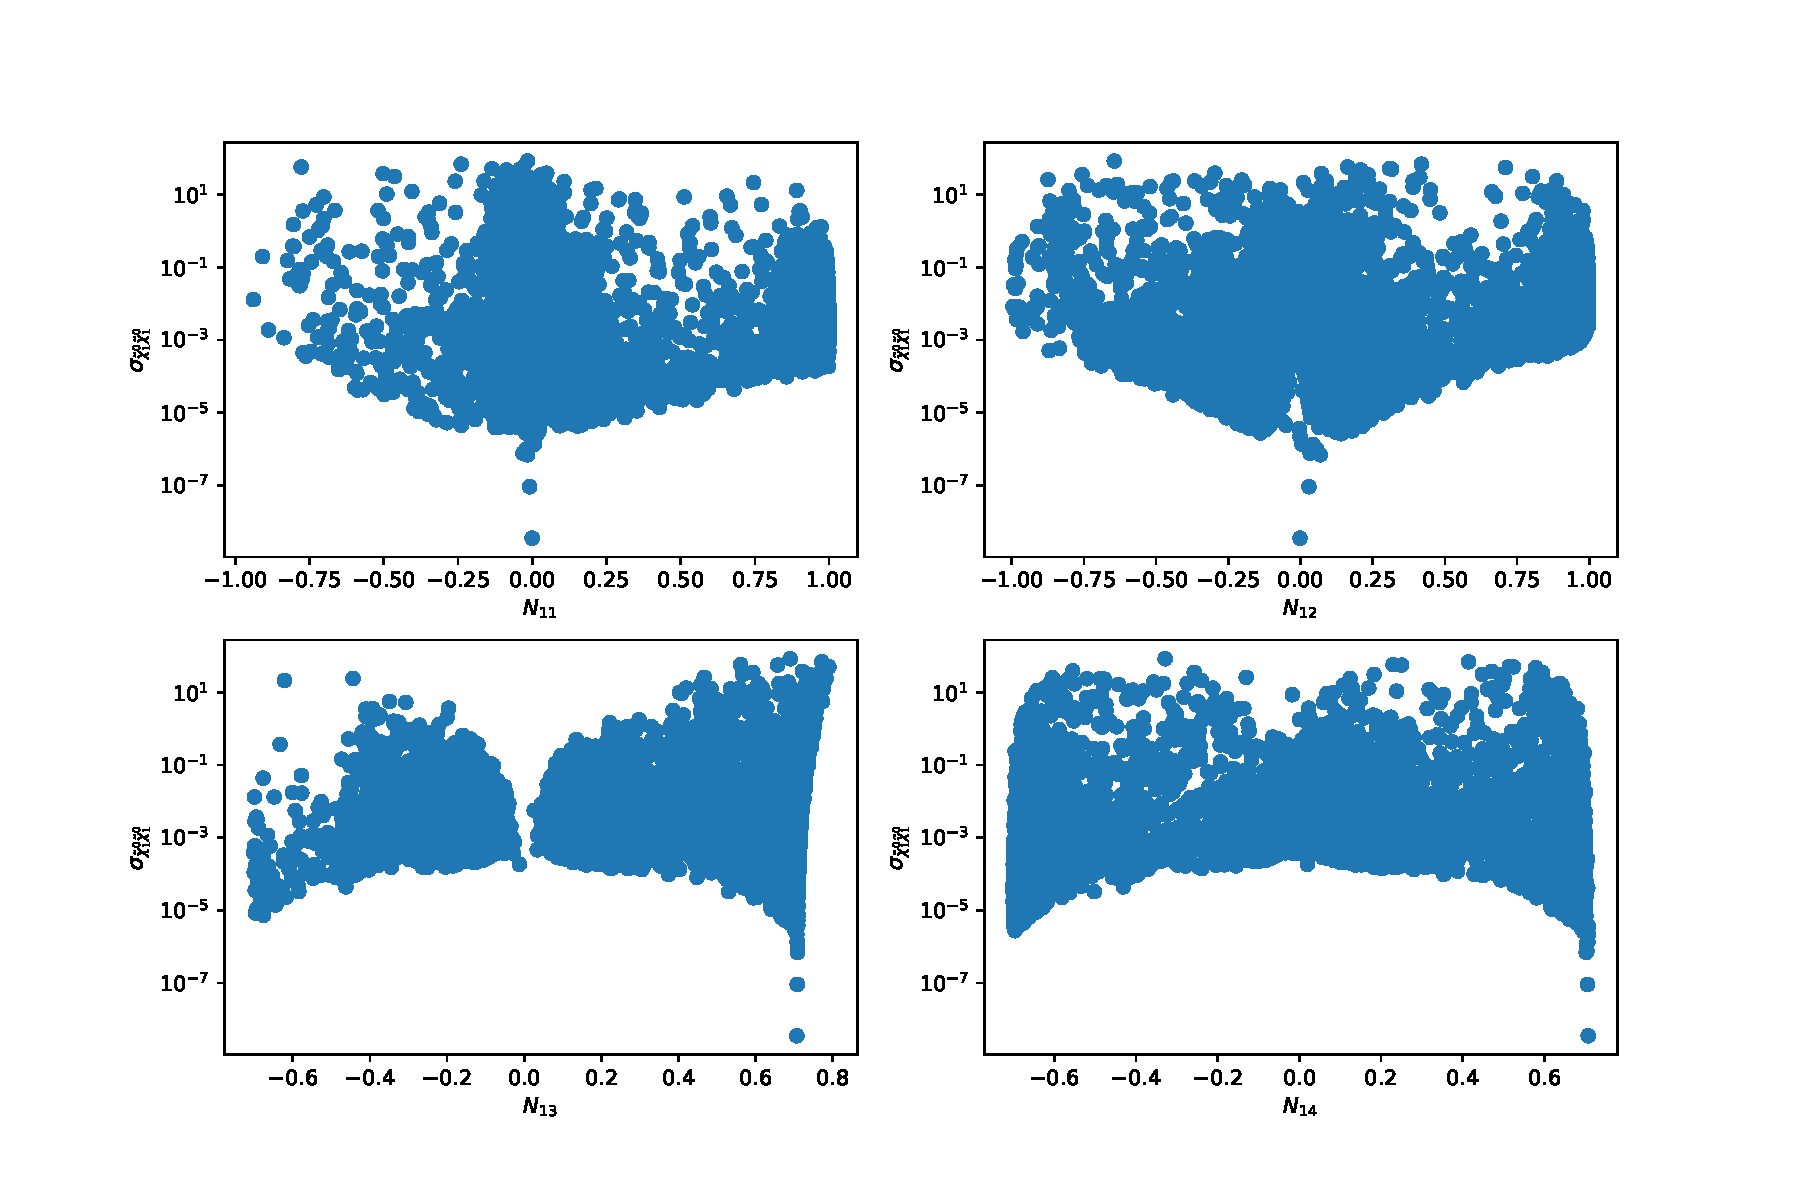
\includegraphics[scale=0.5]{figures/dataset/mixing_angles.pdf}
    \caption{The values of the cross sections $\sigma_{\tilde{\chi}_1^0 \tilde{\chi}_1^0}$ are shown projected onto the axes of mixing angles $N_{1j}$ for $j = 1, 2, 3, 4$. The data is taken from the training data.
    }\label{fig:dataset_mixing_angles}
\end{figure}


\subsection{Data Transformations}\label{sec:data_transform}
We shall briefly discuss how the training data is transformed before training.
The targets in the dataset of NLO cross sections can span several orders of magnitude. For practical training of BNNs, this would require
model parameters that also span several orders of magnitude. The result will usually be numerical overflow and thus unsucessful training of the models.
Therefore, we have chosen to map the targets using the base-10 logarithm, i.e. $y \mapsto \log_{10}(y)$. More generally, we could choose any base-$a$ logarithm. A practical consideration here is that once the model is trained, any prediction it produces must be transformed back using
the inverse mapping to produce a cross section. As we increase the value of $a$, the precision the model's prediction decreases. Thus a small error in log-space 
can result in a large error in what we may refer to as the target space, the larger the value of $a$ is. 
We will explore the performance both in log space using the transformed data and in target space by applying the inverse mapping to the predictions.

\begin{comment}
The models we train will compute predictive distribution for each input and thus must be treated as a stochastic variable. Transformation of its prediction back to target space will thus in practice mean transformation of its sample mean and variance. Denote $f = \log_{10}(y)$ as the targets in log space for a moment, which we regard as a stochastic variable. Let $\mu_f$ be the expectation and $\sigma_f^2$ the variance of the predictive distribution in log space. Let $y = 10^f$ be the corresponding stochastic variable in target space. We need a way to compute the variance $\sigma_y$ in target space given the variance in log space. Consider the Taylor expansion
\begin{equation}
    y \approx y(\mu_f) + y'(\mu_f)(f - \mu_f).
\end{equation}
The variance is then
\begin{equation}
    \text{Var}(y) \approx \abs{y'(\mu_f)}^2\text{Var}(f),
\end{equation}
which imply that to a first order approximation, the propagated error is
\begin{equation}
    \sigma_y \approx \abs{y'(\mu_f)}\sigma_f.
\end{equation}
Applied to the relationship introduced by our transformation of the targets, this imply
\begin{equation}\label{eq:propagated_error}
    \sigma_y \approx 10^{\mu_f} \ln(10)\sigma_f,
\end{equation}
and our estimation of the target is
\begin{equation}
    \hat{y} = 10^{\mu_f}.
\end{equation}
In practice, we will approximate $\mu_f$ with the sample mean of the predictive distribution and $\sigma_f^2$ with its sample variance. From this we can employ the approximation in eq.~\eqref{eq:propagated_error} to give an estimation of the error of the predicted NLO cross section that a BNN model yields.

\end{comment}
\begin{comment}
    \subsubsection{Error Propagation}
As we discussed in section \ref{sec:data_transform}, we perform the mapping $y \mapsto \log_{10}(y)$ on the targets in the training data. Thus our BNN models will train on targets in log space and its predictions will reside in the same space. Let us denote its predictions as $\hat{y}$ which we treat as a stochastic variable since it produces a predictive distribution given an input $x$. Suppose $\hat{y}_\text{mean}$ is the sample mean of its predictions and $\sigma_{\hat{y}}^2$ is the sample variance. Let us denote $\hat{f} = {10}^{\hat{y}}$ as its prediction transformed back to target space. The differential of $\hat{f}$ is
\begin{equation}
    \dd \hat{f} = \dd \hat{y} \ 10^{\hat{y}} \ln(10).
\end{equation}
Treating $\dd \hat{y} \to \sigma_{\hat{y}}$ and $\dd \hat{f} \to \sigma_{\hat{f}}$ we can approximate the error propagated from log space onto target space as
\begin{equation}
    \sigma_{\hat{f}} \approx \sigma_{\hat{y}} \ 10^{\hat{y}} \ln(10),
\end{equation}
where $\hat{y}$ is understood as the sample mean of the 
\end{comment}

\begin{comment}
    A final aspect we mention is that only $a$ on the form $a = 2^b$ for an integer $b \geq 0$ will yield transformed data that can be represented exactly on a computer. Any other transformation automatically introduces a truncation or rounding error once the transformation is performed which introduces a small systematic error in the training data \textit{before} even training has begun. 
\end{comment}

\subsection{Data Splitting}
\textit{Data splitting} is a common strategy in machine learning to avoid biased model selection and obtain reliable estimates of the performance of the trained models.
The conventional way is to split the dataset $\mathcal{D}$ into three subsets: 
\begin{enumerate}
    \item A training set $\mathcal{D}_\text{train}$. This dataset usually contain the largest chunk of the dataset and is used to train the models.
    \item A validation set $\mathcal{D}_\text{val}$. This dataset is typically the smallest of the bunch and is sometimes used in classical machine learning problems to perform cross-validation or similar methods. The results measured here are typically used to select hyperparameters of the model.
    \item A test set $\mathcal{D}_\text{test}$. This partition is slightly larger than the validation set and is used as an out-of-sample check to measure the performance of a model. 
\end{enumerate}
We have selected to use a division of 80\% training data, 5\% validation data and 15\% test data. The absolute size of the full dataset consists of 14683 datapoints. This is a fairly small dataset for a typical machine learning task where neural networks are used. Neural networks are usually called ``data hungry'' and their performance is typically significantly improved by increasing it large amounts of data. 

\section{Training Methodology}
In this section, we shall explain the methodology used to train and test the BNNs explored in this thesis. We will explain the implementations, selection of models and hyperparameters and performance metrics used.

\subsection{Implementation}
We have utilized the Python libraries {\tt TensorFlow 2.7.0} and {\tt TensorFlow-Probability 0.15.0} to implement the BNNs. 
The implementation itself is available at \url{LEGG TIL URL HER eller SITERING}. Unfortunately, BNNs trained with HMC or NUTS have not been of interest for the majority of the deep learning community. The main focus has been with use of surrogate distributions to develop algorithms that when employed using GPUs spend roughly the same amount of time per epoch as training of classical neural networks. As a result no implementations of BNNs for these kind of samplers have been implemented directly into either framework. Luckily, {\tt TensorFlow-Probability} provides general purpose implementations of the samplers we have discussed hithertho 
which only requires us to define the \textit{unnormalized negative log-target density} (which is the negative potential energy function $-\mathcal{L}$) to utilize the them. Thus, we could have implemented BNNs from a strictly functional programming paradigm. However, to storing BNNs requires storage of more than simply the Markov chain generated by the samplers. Additional information such as the activation function used per layer, nodes used per layer and so on makes it fairly impractical. Consequentially, we created an object-oriented implementation that facilitates the usual kind of conveniences shipped with {\tt TensorFlow} such as the ability to automatically save, load or print the model architecture to screen, and provide error handling, to name a few. The class and its functionality is well-documented and made with the intention to be reused, expanded and modified. We do, however, provide a implementation that only uses functional programming as well.

Both {\tt TensorFlow} and {\tt TensorFlow-Probability} handle execution on NVIDIA GPUs automatically with minimal effort on the user side, which we have utilized to generate our results. We will also provide measurements that indicate the expected speedup gained from using a GPU instead of a CPU for training of BNNs. Some of the results are also generated using the built-in GPU on an M1 Apple Silicon system-on-chip (SoC), since a port of {\tt TensorFlow} that supports execution on this device is available. We will make it crystal clear on what hardware the calculations are performed.


\subsection{Performance Metrics}\label{sec:perf_metrics}
In this section, we will discuss the performance metrics used to benchmark and measure the performance of the models trained in this thesis.
Due to the inherent probabilistic nature of the models trained, any output the model produces will be a distribution from which we can calculate
a sample mean and variance. 
We will introduce a metric to measure the performance of the mean predictions of the BNNs called coefficient of determination and a metric to assess the BNNs ability to yield reliable uncertainties in its predictions called standardized residuals.

\subsubsection{Coefficent of Determination}
The \textit{coefficent of determination}, or the $R^2$-\textit{score}, is used to assess the quality of the predictions of a model in supervised regression tasks. For a dataset $\mathcal{D} = \{(x^{(i)}, y^{(i)})\}_{i=1}^N$, it is given by
\begin{equation}\label{eq:r2_score}
    R^2 = 1 - \frac{\sum_{i=1}^N (y^{(i)} - \hat{y}^{(i)})^2}{\sum_{i=1}^N (y^{(i)} - \bar{y})^2},
\end{equation}
where $y^{(i)}$ denotes the target of an input $x^{(i)}$ and $\hat{y}^{(i)}$ denotes the model prediction and $\bar{y}$ denotes the sample mean of the targets
\begin{equation}
    \bar{y} = \frac{1}{N}\sum_{i=1}^N y^{(i)}.
\end{equation}
The $R^2$-score lies in the range $R^2 \in (-\infty, 1]$ where the larger the value, the better the model predicts. The score is interpreted as the proportion of the variance in the targets that can be predicted from the inputs. The reason we select this metric is that it provides a more reliable interpretation of the prediction quality of our models than other metrics such as mean squared error (MSE), root mean squared error (RMSE) and the mean absolute error (MAE) which can only be used to compare the predictions of models relative to each other \cite{r2_score}. Their values all lie in the range of $[0, \infty)$ where a perfect prediction would yield zero. The lack of an upper-bound on these alternative metrics make them difficult to interpret in a vacuum, a weakness the $R^2$-score does not suffer from. If $R^2 < 0$, the model performs poorly, while of $R^2 \in [0, 1]$, the model explains the variation in the data with $R^2 = 0$ meaning the model cannot explain any of the variance in the targets around their sample mean. A score of $R^2 = 1$ means a perfect prediction.

Note that when we use BNNs to compute the $R^2$-score, we will replace $\hat{y}^{(i)}$ in eq.~\eqref{eq:r2_score} with the sample mean of the predictive distribution computed by the BNNs. 

\subsubsection{Standardized Residuals}
\textit{Standardized residuals} is a transformation of a model prediction given an input feature $x^{(i)}$ and a target $y^{(i)}$. The mapping is defined as
\begin{equation}\label{eq:standardized_residuals}
    z^{(i)} = \frac{y^{(i)} - \hat{y}^{(i)}}{\hat{\sigma}^{(i)}},
\end{equation}
where $\hat{\sigma}^{(i)}$ is the square-root of the sample variance of the model predicitions and $\hat{y}^{(i)}$ is the sample mean of the predictions. The mapping in eq.~\eqref{eq:standardized_residuals} resembles the mapping of a random variable $x \sim \mathcal{N}(\mu, \sigma^2)$ onto the standard Normal distribution $z \sim \mathcal{N}(0, 1)$.


As we discussed in chapter \ref{chap:bayesian_ml}, the fundamental assumption made is that any target $y$ can be decomposed as
\begin{equation}
    y = f(x) + \delta,
\end{equation}
for some true function $f(x)$ and a random noise $\delta$, often taken to be distributed according to a Gaussian distribution. But the noise in the data produced by \texttt{Prospino} in the sample generation is neglible, which means that $y \approx f(x)$. The regression error obtained through the sample variance of the model predictions must therefore be dominated by the variance of the predictive distribution computed by the model itself. Let $\sigma_z^2$ denote the variance of the distribution of the standardized residual. If $\sigma_z > 1$, the model will be considered overconfident in its predictions since the sample variance of the model's predictions are smaller than the variance of the targets around the mean prediction. On the other hand, if $\sigma_z \leq 1$, we consider the model to yield reliable uncertainty estimates. In this case, the model is not considered to be ``underconfident'' but rather ``conservative''. As a visual aid, we will draw in the standard Normal distribution $\mathcal{N}(0, 1)$ with the distibutions obtained with eq.~\eqref{eq:standardized_residuals} for reference. If the distribution lies largely on the ``inside'' of $\mathcal{N}(0, 1)$, we can consider it as a conservative model to an approximation. But note that the distribution may have longer ``tails'' than the usual Normal distribution and thus 
$\sigma_z > 1$ is possible even if the majority of the distribution lies inside the Normal distribution.

\subsection{Potential Scale Reduction}
The potential scale reduction $\hat{R}$ \cite{rhat} is a quantity used for convergence diagnostic purposes of Markov chains. Using it directly on the posterior weights of Bayesian neural networks is difficult due to unidenfiability of neural network parameters. The diagnostic may indicate that the samples of a neural network has not converged to its stationary distribution as a result. It is therefore better used on a space of scalar functions $f(\theta)$ of the model parameters $\theta$.
Consider $M$ independent Markov chains numbered by $m \in \{1, \ldots, M\}$ and let each chain consist of $N$ samples numbered by $n \in \{1, \ldots, N\}$. 
Let us denote $\theta_{mn}$ as the $n$-th sample of the $m$-th Markov chain.
Furthermore, we denote $f_{mn} \equiv f(\theta_{mn})$. Then the potential scale reduction is defined by the following equations.
\begin{equation}
    \bar{f}_m \equiv \frac{1}{N}\sum_{n=1}^N f_{mn},
\end{equation}
which denotes the sample mean of the $m$-th chain. Let us define the sample mean across all chains as
\begin{equation}
    \bar{f} \equiv \frac{1}{MN}\sum_{m=1}^M\sum_{n=1}^N f_{mn}.
\end{equation}
Then the sample variance \textit{across} the chains is given as
\begin{equation}
    \frac{B}{N} \equiv \frac{1}{M-1} \sum_{m=1}^M (\bar{f}_m - \bar{f})^2.
\end{equation}
The sample mean of the sample variance \textit{within} the chains is
\begin{equation}
    W \equiv \frac{1}{M}\sum_{m=1}^M \frac{1}{N-1}\sum_{n=1}^N(f_{mn} - \bar{f}_m)^2 = \frac{1}{M(N-1)}\sum_{m=1}^M \sum_{n=1}^N (f_{mn} - \bar{f}_m)^2.
\end{equation}
Define further
\begin{equation}
    \sigma_+^2 \equiv \frac{N-1}{N}W + \frac{B}{N},
\end{equation}
which if the chains are initiated \textit{from} the stationary distribution, will yield an unbiased estimate of the variance of the distribution.
Then the potential scale reduction is given by 
\begin{equation}
    \hat{R} \equiv \frac{M + 1}{M}\frac{\sigma_+^2}{W} - \frac{N - 1}{MN}.
\end{equation}
The interpretation of $\hat{R}$ is as follows. If $\hat{R}$ is larger than one, then more simulations can be performed to further bring each chain closer to the stationary distribution. If $\hat{R}$ is close to one, then each $m$ chains of $n$ samples are close to the stationary distribution. A common heuristic is to assume the chains have converged sufficiently if $\hat{R} < 1.1$ \cite{convergence_diagnostics}.



